\documentclass[main.tex]{subfiles} 
\begin{document}

\section*{Drøfting}

\subsection*{Repesentasjoner}

Til denne oppgaven har jeg valgt å fokusere på kompetansemål relatert til organisk kjemi. Ofte når elever blir introdusert til organisk kjemi er deres første stoppested ved hydrokarboner og navnsetting av hydrokarboner. Gjennom egen praksiserfaring har jeg opplevd dette som en fin introduksjon til det overordnede temaet oragnisk kjemi. Mange elever opplever initielt vansker med navnsetting av blant annet hydrokarboner, mens noen elever opplever innføringen systematisk og klarer fort å beherske navnsetting og beveger seg videre til andre temaer som alkoholer, karboksylsyrer og karbohydrater. Progresjon til disse temaene har en naturlig overgang, fra å lære seg å navnsette hydrokarboner til å utvide de kjemiske forbindelsene ved å legge til hydroksylgrupper og karboksylgrupper. Her kan vi se at elevene må ha en god begrepsforståelse for at de skal kunne danne en fagovergripelig forståelse. Mork og Erlien skriver at begreper er kanskje det området i naturfag som forårsaker flest problemer for læring, fordi noen begreper kan være veldig abstrakte (\citeNP[s. 24]{moer10}).
\newline\newline
Elever som har vansker med å navnsette og skille hydrokarboner, alkoholer og organiske syrer, har også ofte problemmer med å visualisere de kjemiske forbindelsene, eller tolke strukturformelen. Det blir enda vanskeligere for disse elevene når alkaner, alkener og alkyner, det vil si enkelt, dobbelt og trippelbindinger innføres. Da må de i tillegg holde oversikt over bindinger og hvor hydrogenatomer kan forbinde seg til karbon-atomet. Derfor er det viktig for både de lavt presterende -og høytpresterende elevene at de kan ha gode illustrasjoner som kan visualisere teorien på en forståelig vis. Dersom målet med undervisningen er at alle elever skal forstå det som undervises er det da viktig å treffe  hver enkelt elev som har ulik tilnærming til stoff og gi hver elev mange erfaringer innenfor samme tema (\citeNP[s. 32]{froy10}). 
\newline\newline
Bruk av interaktive programer (f.eks flash basert nettside Lokus - se figur \ref{fig:lokus}) kan ha en gunstig virkning og hjelpe de lavt presterende elevene med å skape motivasjon. Et annet virkemiddel er et molekylbyggesett. Her kan elevene få en fysisk tilknyttning til strukturene de leser om og navnsetter gjennom førstehåndserfaring (\citeNP[s. 111]{froy10}). Gjennom min egen praksiserfaring har jeg opplevd at bruk av molekylbyggesett kan være motiverende og innlysende. Når elever forsøker å lage fysiske bindinger mellom karbonatomer og andre atomer ser mange at det er begrenset hvordan disse bindingene kan skapes. Derfor har slike byggesett en didaktisk betydning for elevene.\newline

\begin{figure}[h!]
\centering
    \begin{subfigure}{.5\textwidth}
    \centering
    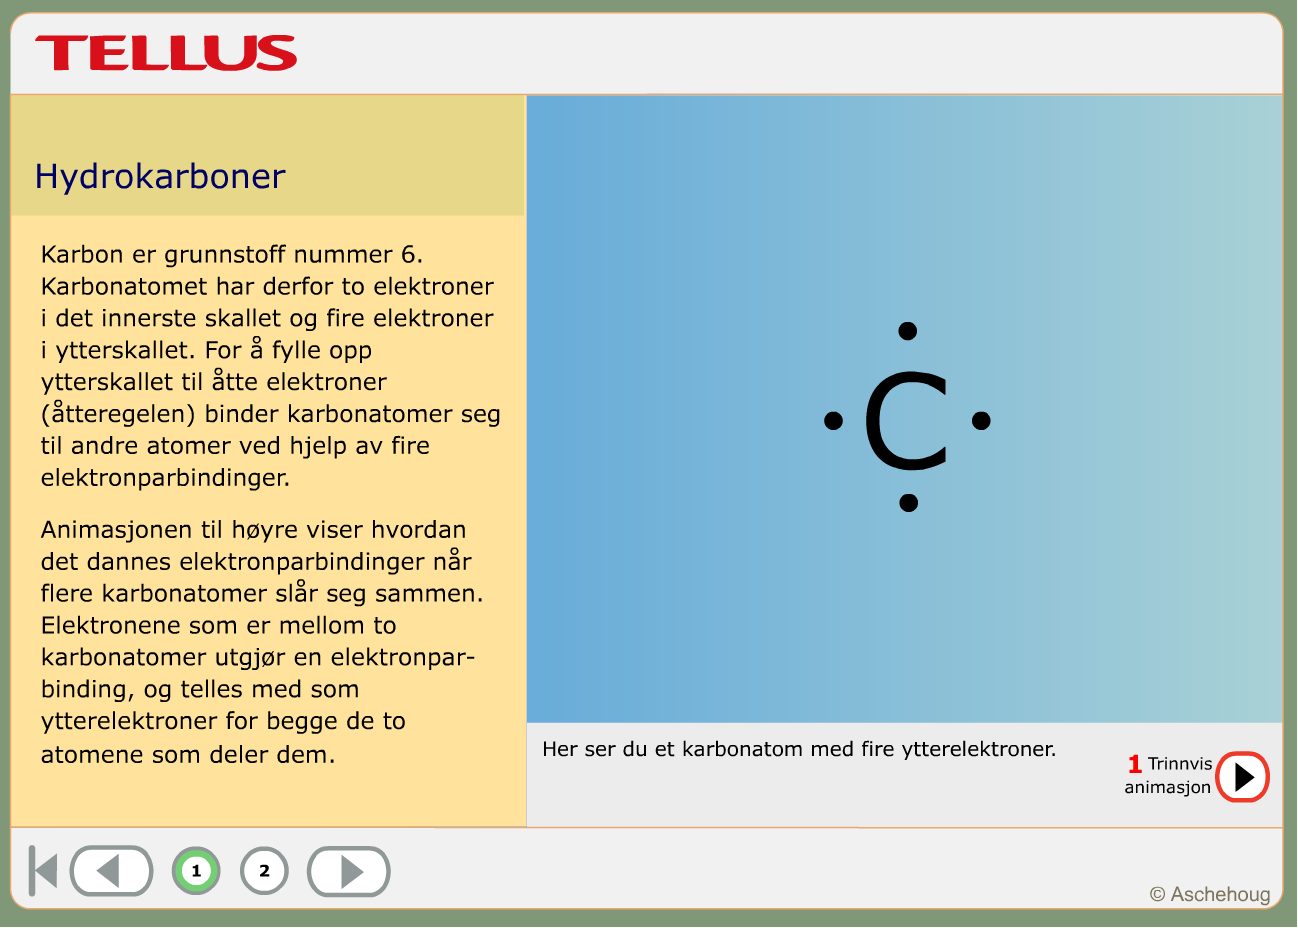
\includegraphics[scale = 0.20]{../figures/lokus1.png}
    \end{subfigure}%%
    \begin{subfigure}{.5\textwidth}
    \centering
    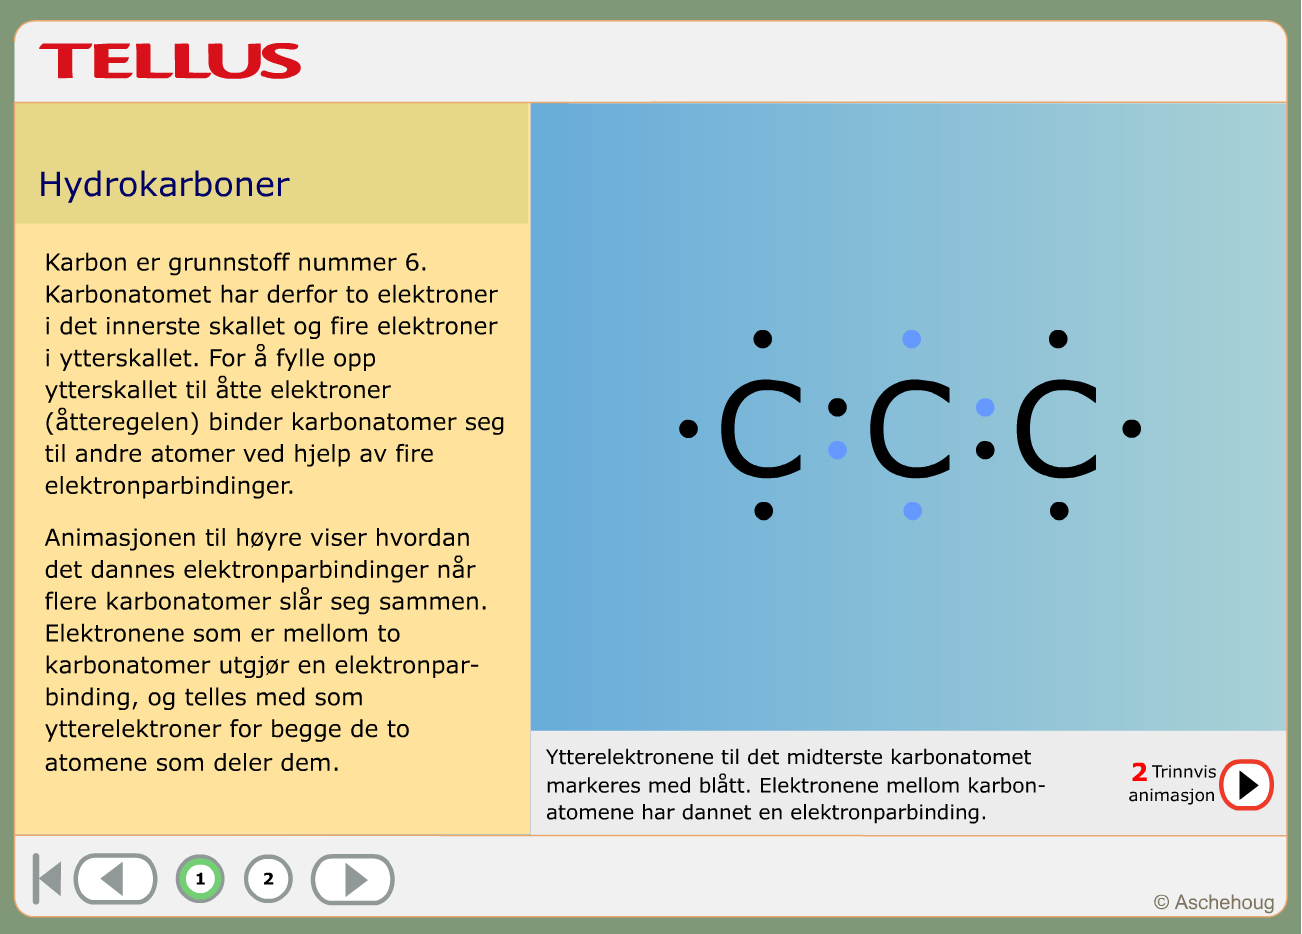
\includegraphics[scale = 0.199]{../figures/lokus2.png}
    \end{subfigure}
    \begin{subfigure}{.5\textwidth}
    \centering
    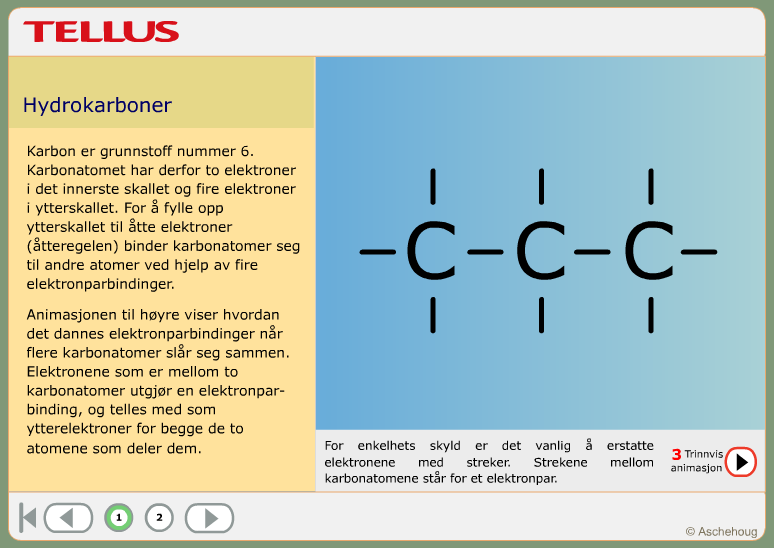
\includegraphics[scale = 0.34]{../figures/lokus3.png}
    \end{subfigure}%%
    \begin{subfigure}{.5\textwidth}
    \centering
    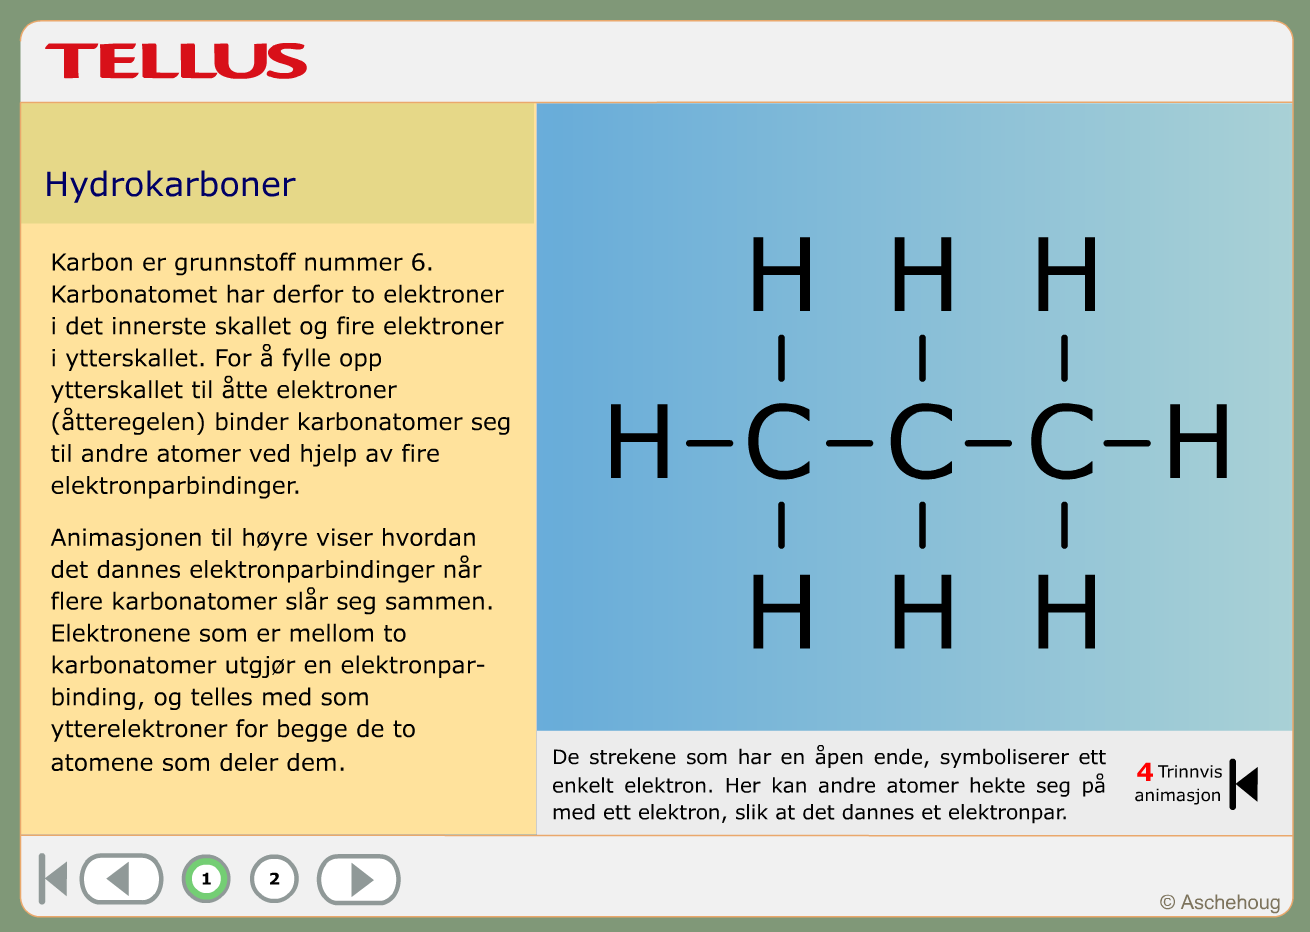
\includegraphics[scale = 0.199]{../figures/lokus4.png}
    \end{subfigure}
    \caption{Interaktiv forklaring for elektronparbindinger når flere karbonatomer slår seg sammen. Kilde: 
    \protect\url{http://www3.lokus.no/flashEmbedder.jsp?contentItemId=52275952&selectedLanguageId=1&title=hydrokarboner}}
    \label{fig:lokus}
\end{figure}

\begin{figure}[h!]
\centering
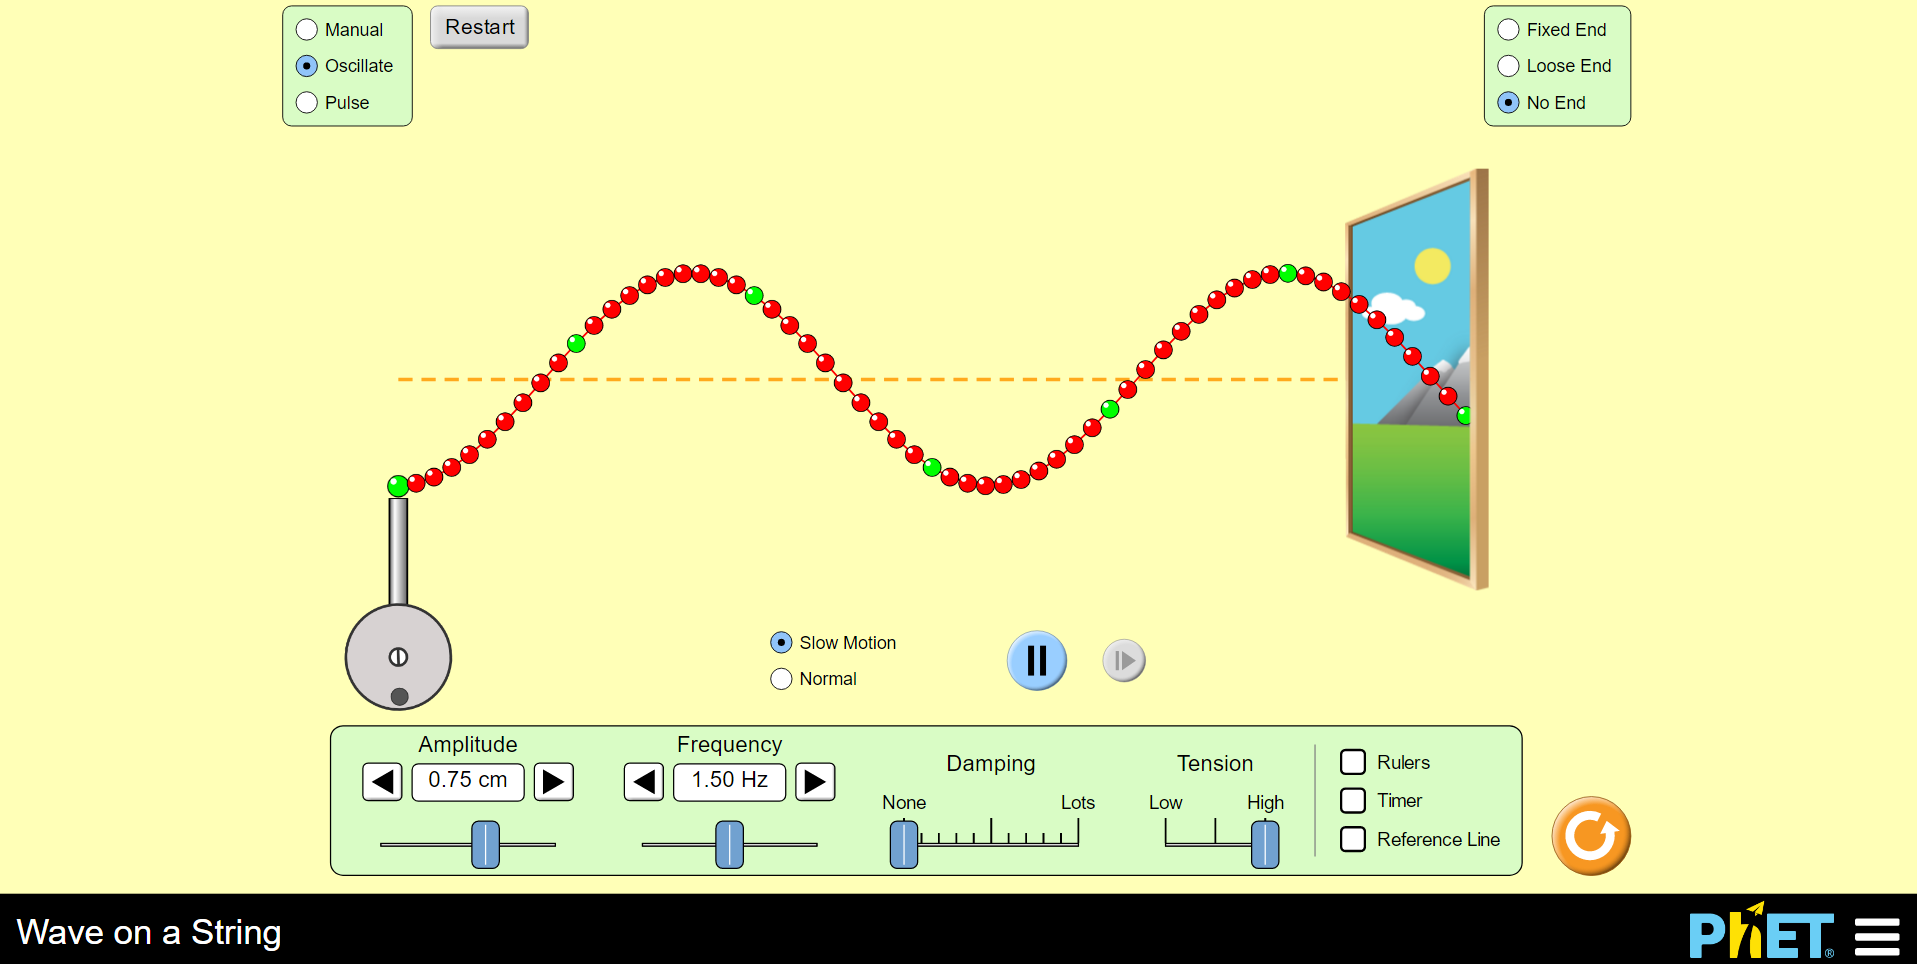
\includegraphics[scale = 0.25]{../figures/wave.png}
\caption{Interaktiv simulering av en oscillerende streng. Kilde: 
\protect\url{https://phet.colorado.edu/sims/html/wave-on-a-string/latest/wave-on-a-string_en.html}}
\label{fig:wave}
\end{figure}

\hspace{-6mm}I denne oppgaven er fokuset rundt tekster og illustrasjoner for å skape en tilpasset opplæring. Her har jeg snakket om en spesifikk naturfagstime som hovedsakelig dreier seg om innføring av hydrokarboner og navnsetting av hydrokarboner ved hjelp av strukturformel. Gjennom andre temaer jeg har undervist jeg har erfart at bruk av simuleringer (f.eks flash basert nettside PhET Interactive Simulations : se figur \ref{fig:wave}) kan også skape variasjon og motivasjon blant elever på tvers av faglig nivå. Jeg brukte simuleringen i figur \ref{fig:wave} til å koble temaet elektromagnetisk stråling til frekvens og bølgelengde av en oscillerende streng. Det viste seg at elever som ellers ikke er aktive i timen viste stor intresse og forsøkte å få simuleringen til å virke autentisk ved å endre på parametere.\newline

\begin{figure}[h!]
\centering
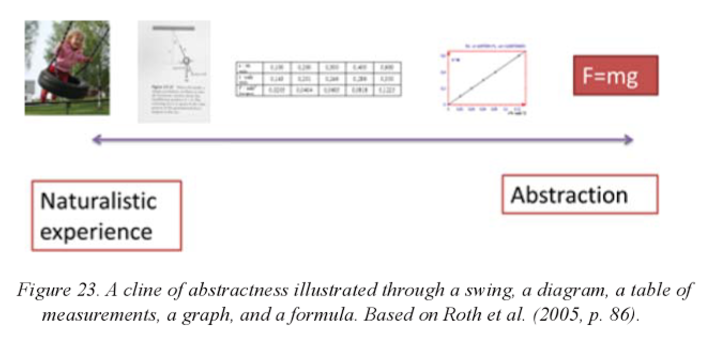
\includegraphics[scale = 0.6]{../figures/knain.png}
\caption{Grad av abstraksjoner. Kilde: \protect\citeA[s.80]{knai15}}
\label{fig:knain}
\end{figure}

\hspace{-6mm}\citeA[s. 80 - 81]{knai15} skriver at slike representasjoner binder tekst og illustrasjoner fra bøker til en direkte erfaring eller video som viser. Han illustrer dette (se figur \ref{fig:knain}) ved å sette direkte erfaring på en side av abstraksjonsskalaen til ren abstraksjoner (som f.eks formler) på den andre siden. Fra lærerens side kreves det god faglig kompetanse for å finne ut om en simulering eller animasjon fremstiller en naturfaglig prosess riktig. En faglig dyktig lærer ser ofte mange muligheter og er kreativ når det gjelder valg av metoder og tilrettelegging (\citeNP[s. 148]{moer10}). For eleven innebærer valg av gode representasjoner økt evne til å lese en tekst eller lærebok (\citeNP[s. 84]{knai15}).


\subsection*{Kompetansemål}
For eksempel diskutere er et høyt kompetansenivå, der eleven kan trekke sammnenhenger og redegjøre for sine tanker om en problemstilling. I motsetning er å beskrive et middels kompetansenivå (i Bloom's taksonomi).


Gjennom noen av mine samtaler med elever, oppdaget jeg fort at det var få som trakk forbindelsen mellom egen læring og koblingen til kompetansemålene. For undervisere regnes det som en god praksis at elevene er alltid bevisste om hvorfor de lærer det de lærer og hvor de er på vei. \citeA[s. 136]{klet13} beskriver en god undervisningsseksens der lærere klarer å balansere mellom tilegnelses-, utprøvings-, og konsolideringssituasjoner. Ifølge Klette har norske klasserom ensidige tendenser i bruken av varierte arbeidsmåter. Slik det kan ses fra figur \ref{fig:odeg10}, er det for eksempel lite konsolideringssituasjoner. Lærernes metalæringsaktiviteter regnes som særlig avgjørende for å sikre elevenes læring (\citeNP[s. 186]{klet13}). Å bruke dette som et fast organiserende prinsipp, blir derimot sjelden gjennomført (\citeNP[s. 26]{odeg10}). Dermed er det viktig å koble inn kompetansemålene og jobbe målrettet mot høyere kompetansenivå. Dette vil fremme læing hos eleven og gi eleven en pekepinn på hvor hen må ta tak.
\begin{figure}[h!]
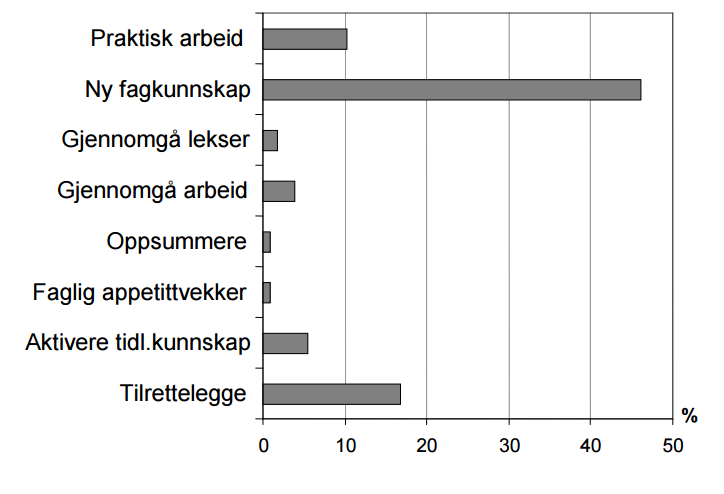
\includegraphics[scale = 0.6]{../figures/undervisnings_aktivitet.png}
\caption{Oversikt over naturfaglærernes undervisningstilbud til elevene fra PISA+ studie. Kilde: 
\protect\citeA{odeg10}.}
\label{fig:odeg10}
\end{figure}



\subsection*{Gruppearbeid}

Et funn innenfor utdanningsforskning er at hjemmebakgrunn har sterk sammenheng med elevers faglige prestasjoner (\citeNP[s. 176]{berg16}). Et viktig mål for norsk skole er å utjevne sosiale forskjeller mellom elevene. Bergem fremhever faktoren som styrker elevenes hjemmebakgrunn og deres prestasjoner, er hovedsakelig lekser. Hans undersøkelse viste at jo flere lekser som gis, \emph{jo mer øker betydningen av hjemmebakgrunn for elevenes prestasjoner} (\citeNP[s. 176]{berg16}). Fosse skriver at utstrakt bruk av individuelle metoder kan føre til manglende inkludering. Siden individualiserte metoder krever stor selvstendighet hos elevene, vil elever som har vansker med selvregulært læring falle utenfor (\citeNP[s.431]{foss14}). 

\citeA[s. 176]{klet13} viser til viktigheten av at lærere legger til rette for ``systematisk trening, øvelse og bruk av naturfaglige begreper for å utvikle elevenes naturfaglige forståelse''. Muntlige ferdigheter er en av grunneleggende ferdigheter i naturfag. I læreplanen står det blant annet: ``Utviklingen av muntlige ferdigheter i naturfag går fra å kunne lytte og samtale om opplevelser og observasjoner til å kunne presentere og diskutere stadig mer komplekse emner''. I den sosiokulturelle tradisjonen rettes fokus mot læring i felleskap før kunnskap blir internalisert på individnivå (\citeNP[s. 90]{salj13}). Blant annet inkluderer dette arbeid i grupper.


I et sosiokulturelt læringsperspektiv skjer differensiering i sosiale læringssituasjoner (\citeNP{brgu16}), hvor det består det i å veilede elevene i den nærmeste utviklingssonen.\footnote[2]{Den \emph{nærmeste utviklingssonen} beskriver en sone som ligger i mellom en elevs kognitive ferdigheter, dvs. hva de kan oppnå selvstendig uten hjelp, og elevens potensielle utvikling, dvs. hva en elev kan få til eller forstå gjennom veiledning (\citeNP[s. 125]{bta98}; \citeNP[s. 75]{salj13}; \citeNP[s. 154]{mang13}).} Bruk av ''scaffolding`` eller stillasbygging (\citeNP{bta98}) er da viktig for å knytte fagbegreper og teori til elevenes forkunnskaper.

Design av gruppeoppgaven bør utformes slik at
elevene er nødt til å jobbe sammen. Oppgaven bør ikke være så enkel at elevene kan jobbe
individuelt med deloppgavene, slik at det ikke er noen nødvendighet for elevene å jobbe sam-
men. Tilsvarende bør oppgaven ikke ha så høy vanskelighetsgrad slik at de ikke klarer å danne
forståelse eller mening. En gruppeoppgave er da en oppgave som individet ikke klarer å utføre
alene og som krever kollaborasjon. Åpne oppgaver er bedre egnet enn lukkede hvor fokuset er
å finne en riktig svar. Dette er kanskje grunnen til at en sterk elev kan dominere samtalen 
(\citeNP[s. 31]{meli07}).

Gode fagsentrerte samtaler mellom elever (eller faglige samtaler med lærer) hvor elever bruker egne erfaringer og språk for å oppnå faglig forståelse hjelper til å skape bro mellom praksis og teori (\citeNP{odeg10})

\end{document}